\chapter{Calculation of Hoop Stress}
\label{Hoop stress}

In order to maintain positive pressure inside the envelope, three main loadings are considered to estimate the internal over pressure ($ \Delta P $) viz., the loading due to dynamic pressure, aerodynamic loading, and hydro-static pressure as suggested by Gupta \& Malik \cite{gupta2002envelope} . A brief description of these three components of the module is as given below.

\textbf{Dynamic Pressure}: Dynamic pressure loading acts on the front portion of the aerostat envelope and tries to make a depression on the envelope surface, its diameter depends on the region of highly stressed area which is normally 7 to 9 \% of the envelope length. To maintain the shape of the envelope, the internal pressure is kept slightly higher than dynamic pressure, normally 15\% as suggested by Gupta \& Malik \cite{gupta2002envelope} as per Eq. \ref{dyn}
\begin{equation}
\label{dyn}
\Delta P_{dyn} = 1.15 \bigg( \frac{1}{2} \rho_{air} v^{2} \bigg)
\end{equation}

\textbf{Aerodynamic Pressure}: Aerodynamic pressure loading results from applying the stability conditions to the airship. Coefficient of pressure, as observed normally for airship profiles is in the range of 0.30 to 0.35 from the leading edge, but normally for such shapes, it is assumed at the maximum diameter. is used for calculating the pressure due to this loading.

\begin{equation}
\label{aer}
\Delta P_{aer} = c_{p} \bigg( \frac{1}{2} \rho_{air} v^{2} \bigg)
\end{equation}

\textbf{Hydrostatic Pressure}: Hydrostatic pressure loading is due to the difference between the height of the top and bottom of aerostat and could be quite substantial of the aerostat diameter in large. The hydrostatic pressure as observed at mean centerline axis of the envelope is calculated at maximum diameter using:

\begin{equation}
\label{hyd}
\Delta P_{hyd} = \frac{1}{2} (\rho _{air} - \rho_{He} ) g D_{c}
\end{equation}
The sum of pressure due to these three loadings gives the total required internal pressure. Since the aerostat envelope diameter is more than twenty times of the thickness of the material; it can be considered as a very thin shell and hence hoop stress is calculated in terms of the circumferential unit load as shown in Eq. \ref{sum_delta}
\begin{equation}
\label{sum_delta}
\Delta P = \Delta P_{dyn} + \Delta P_{aer} + \Delta P_{hyd}
\end{equation}
To estimate the longitudinal stress ($ \sigma _{l} $ ) and the circumferential hoop stress ($ \sigma _{h} $) developed in an envelope, an equivalent cylindrical envelope is considered, having the same surface area and volume as the actual airship envelope, as shown in Fig \ref{Stress representation in envelope}

\begin{figure}[H]
	\centering
	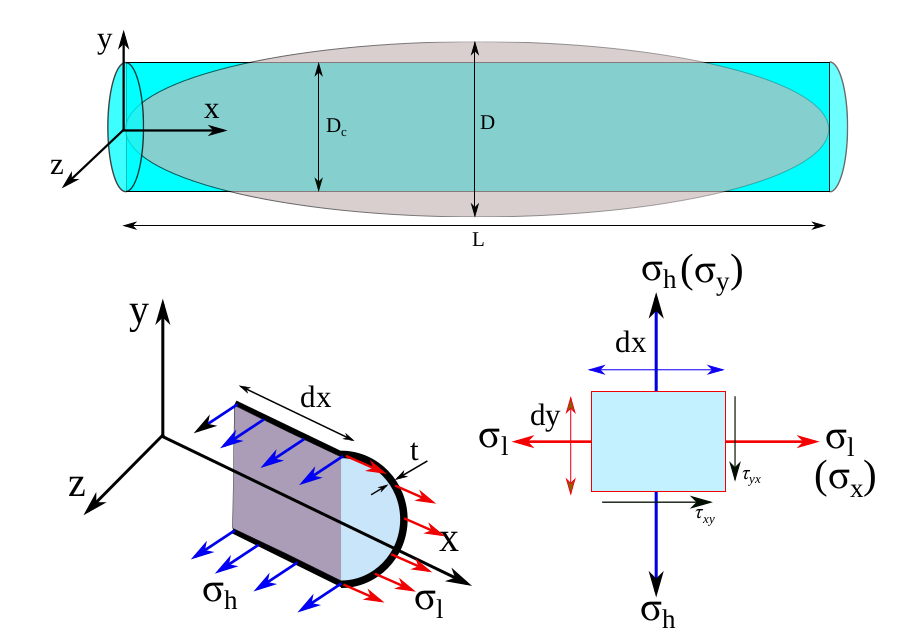
\includegraphics[width=0.7\linewidth]{von_mises/stress_rep_envelope.png}
	\caption{Stress representation in envelope}
	\label{Stress representation in envelope}
\end{figure}
Hence, $ \sigma _{l} $ and $ \sigma _{h} $ developed in an envelope are estimated as:

\begin{equation}
 \sigma _{h} = \frac{\Delta P D_{c}}{2}
\end{equation}

\begin{equation}
\sigma _{l} = \frac{\Delta P D_{c}}{4}
\end{equation}

To maintain the aerodynamic shape and rigidity of an airship envelope some pressure difference ( $ \Delta P^{'} $ ) is also needed, which can be determined by bending moment estimation.

\subsection{Bending Moment Calculation}

An empirical relation for maximum bending moment given by FAA \citenum{cheeseman1999} can be expressed as:
\begin{equation}
\label{moment_eqn}
M = 0.029 [1 + (f-4)(0.5624L^{0.02} - 0.5)]\ \rho _{air} . u . v . V_{env} L^{0.25}
\end{equation}
Where D, is the diameter of airship envelope with the where u and v are the gust and wind velocity respectively. Eq. \ref{moment_eqn} is valid for fineness ration between 4 to 6. For fineness ratio less than 4, f can be assumed as 4.
The point at which the maximum bending moment occurs, i.e., near the center of gravity, $ \sigma _{l} $ at the top of this must be greater than or equal to zero. Therefore, the equation for $ \sigma _{l} $ can be written as:

\begin{equation}
\label{eqn_for_sima_l}
\sigma _{l} = \dfrac{ \Delta P^{'} \pi R^{2} } {2 \pi R } - \frac{MRT}{I} \ge 0
\end{equation}

Where R is the radius of airship envelope at the point of maximum bending. \textit{t} is the thickness the envelope material. \textit{I} is the second moment of area, which has the value of $ \pi R^{3} t $. Minimum pressure required $ \Delta P^{'} $ to maintain the shape of the envelope can be calculated as:

\begin{equation}
\Delta P^{'} = \frac{16M}{\pi D^{3} }
\end{equation}

Where D is the diameter of airship envelope with the assumption that, the location of maximum bending is same as the location of maximum diameter. Total differential pressure ∆P t can be obtained as:
\begin{equation}
\Delta P_{t} = max(\Delta P , \Delta P ^{'})
\end{equation}
In that case, $ \sigma _{h} $ and  $ \sigma _{l} $ can be calculated as:

\begin{equation}
\sigma _{h} = \frac{\Delta P D_{c}}{2}
\end{equation}
\begin{equation}
\sigma _{l} = \frac{\Delta P D}{4} + \frac{4M}{\pi D^{2} }
\end{equation}

\textbf{von-Mises Stress Calculation}: From the principle stresses, von-Mises stress can be expressed as:

\begin{equation}
\sigma _{v} = \Bigg[ \frac{(\sigma _{1}  - \sigma _{2})^2 + (\sigma _{2}  - \sigma _{3})^2 + (\sigma _{3}  - \sigma _{1})^2 }{2}   \Bigg]^{\frac{1}{2}}
\end{equation}

Stresses are considered only in 2-D planes due to very low thickness of envelope compared to its diameter. Therefore $ \sigma _{3} $ = 0, which simplifies the equation as:

\begin{equation}
\sigma _{v} = \sqrt{\frac{(\sigma _{1} - \sigma _{2})^{2} + \sigma _{1} ^{2} + \sigma _{2} ^{2}}{2}}
\end{equation}

\begin{equation}
\sigma _{v} = \sqrt{\sigma _{1} ^{2} + \sigma _{2} ^{2} - \sigma _{1} \sigma _{2}}
\end{equation}

\section{Shape for minimum hoop stress}
An octave function namely $ Von_Mises.m $ has been written incorporating the concepts of section \ref{Hoop stress}. This function gives the value of von-Mises stress ($ \sigma _{v} $) given the values of design parametres shown in Table \ref{Degign space }. The optimal results obtained are as follows:
\begin{table}[H]
	\centering
	\caption{Optimal solution obtained for miminum $ \sigma _{v} $}
	\label{Optimal solution obtained for mimimum sigma_v}
	%\begin{ruledtabular}
	\begin{tabular}{lc}
		\hline \hline
		Design Parameters & Optimal value for minimum $ C_{DV} $    \\ \hline \hline
		
		$ Point\ of\ Max.\ Dia., m$ & 0.44960      \\  
		$ Nose\ Radius, r _{o} $ & 0.38316    \\
		$ Tail\ Radius, r _{1} $ & 0.23247     \\  
		$ Prismatic\ Coeff., C _{p }$ & 0.60598 \\
		$ Fineness\ Ratio, \frac{l}{d} $ &4.28392 \\
		$Scaling\ in\ Y\ direction,\ scale\_y$ &1.50423 \\ \hline \hline
		
		$ von-Mises\ stress\  \sigma _{v}  $ & \\
		\hline \hline
	\end{tabular}
	%	\end{ruledtabular}
\end{table}

%%% Local Variables: 
%%% mode: latex
%%% TeX-master: "../mainrep"
%%% End: 
